% diffuse/intro.tex          pdflatex ZhCvGo15

% Predrag                               24jul2016
% Predrag                                3dec2015
% Tingnan                                2nov2015
% Predrag initial draft                 21nov2014
%         extracted from ChaosBook.org
% \Chapter{diffusion}{2apr2014}{Deterministic diffusion}

% \section{Introduction}

The Lorentz gas is one of the simplest dynamical syst\-ems that exhibit
deterministic diffusion.
Proposed by H. A. Lorentz\rf{Lorentz1905} in 1905, the model has been not only
useful in studying thermal and diffusive properties of dilute electron gases, but
also to address fundamental questions on how ergodicity arises from determinism
in dynamical formulations of statistical physics.
Lorentz gas models the motion of a light molecule within a large number of heavy
scatterers by a point particle at $x(\zeit)$ bouncing off a stationary collection
of reflecting bodies.
It is called ``gas,'' because one can think of it as consisting of any number of
point-like fast ``light molecules'' interacting only with the stationary ``heavy
molecules,'' but not among themselves.
Lorentz assumed a random distribution of heavy scatterers; description of such
gases requires statistical assumptions about the distribution of scatterers.

A {\em periodic} Lorenz gas (configuration of scatterers invariant under a
discrete group of translations of the plane), however, is amenable to pure
deterministic description.
As the scatterer array is built up from defocusing surfaces, it is one of the
simplest hyperbolic Hamiltonian dynamical systems that exhibits chaos and
deterministic diffusion, see \reffig{fig-chaoticBouncing}.
Ergodic properties of periodic Lorenz gases were first studied in 1970 by
Sinai\rf{Sinai70}, and their diffusive properties have been extensively studied
ever since%
\rf{Gallavotti75,BunSin80,BunSin81,MacZwa83,Bunimovich85,GasNic90,BuSiCh90};
for a recent review  see Dettmann\rf{Dettm14}.
%
\begin{figure}[htbp]
	\begin{center}
		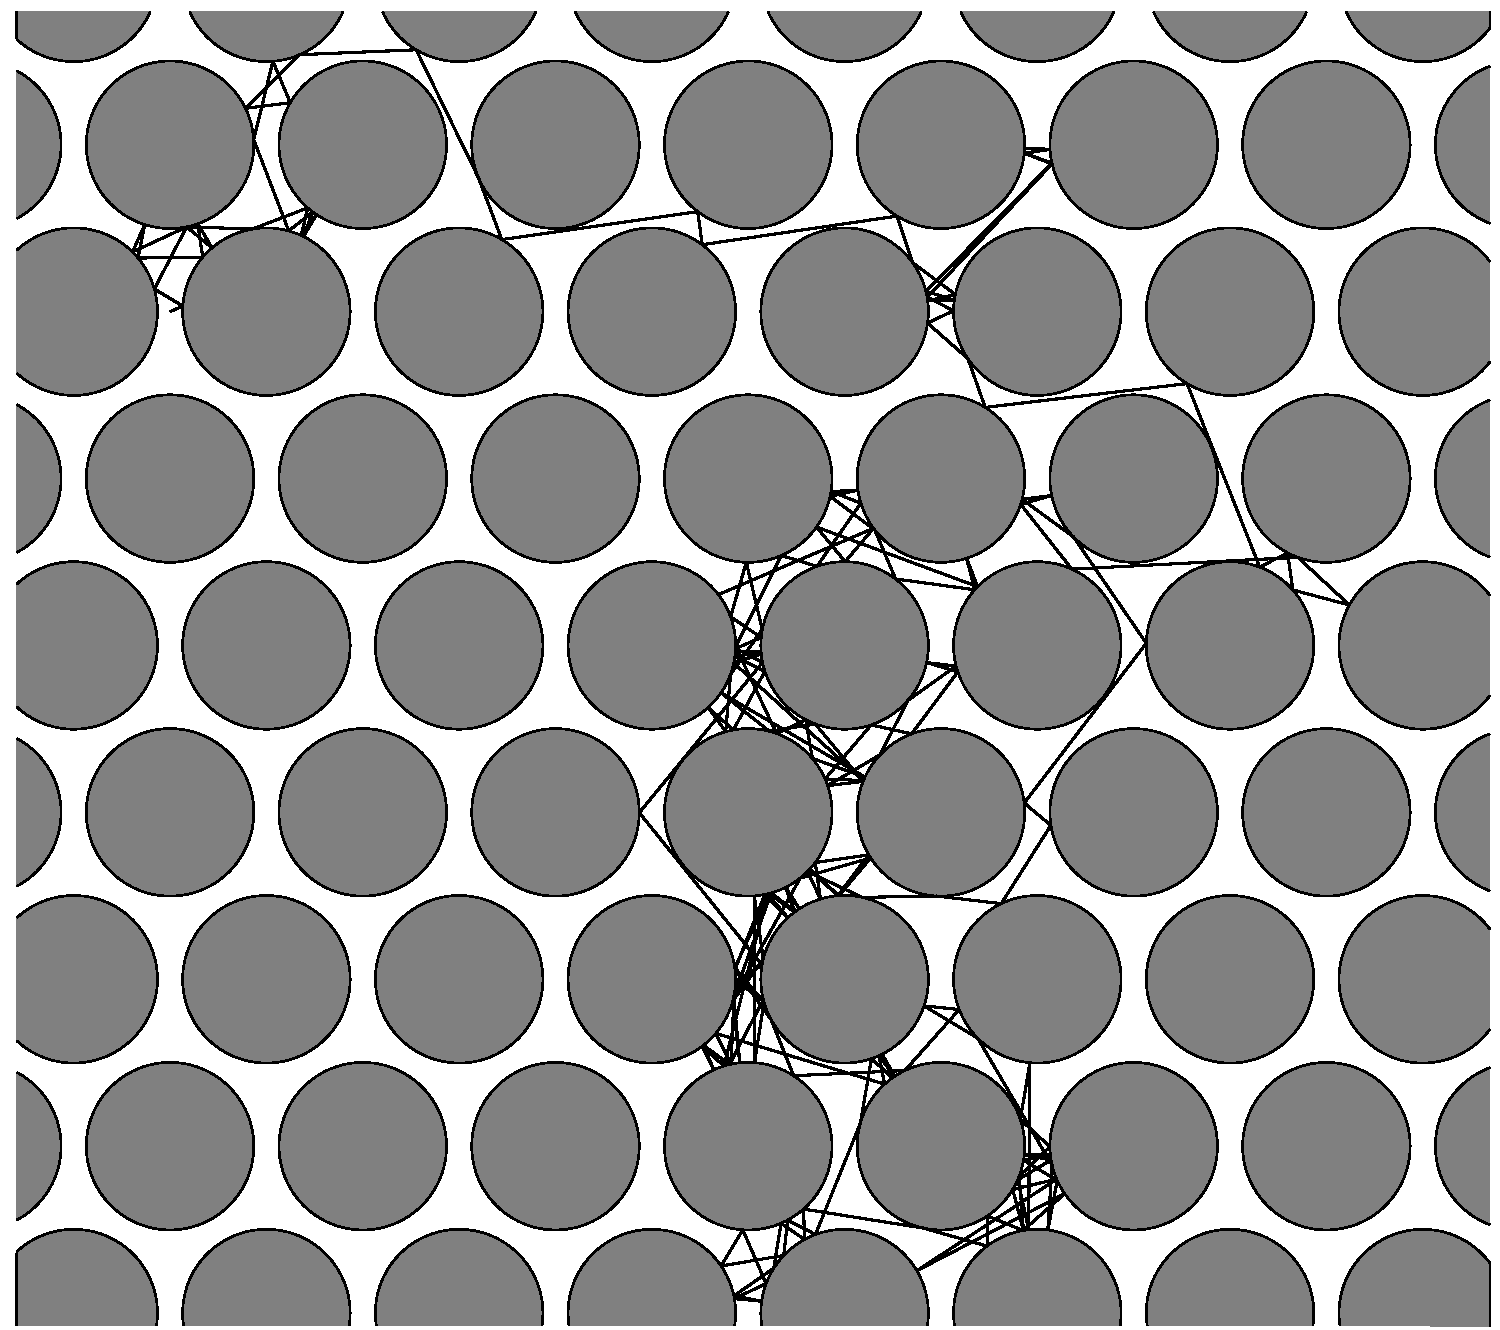
\includegraphics[width=0.45\textwidth]{diffuseChaoticBouncing}
	\end{center}
	\caption[]{\label{fig-chaoticBouncing}
A chaotic trajectory of a finite horizon Lorentz gas point particle bouncing in a
hexagonal planar array of disks. The disks are spaced sufficiently closely so that
no free flight segment is of infinite length.
	}
\end{figure}
%
In this literature
the diffusion constant is defined by
the Einstein-Green-Kubo long-time limit
\beq
D = \lim_{\zeit \to \infty} \frac{\expct{|x(\zeit)-x(0)|^2}}{4\zeit}
\ee{EGKdiff}
Since Sinai's  1970 investigations, theory of dynamical systems has yielded new
sets of microscopic dynamics formulas for macroscopic observables such as the
diffusion constant.
The classical Boltzmann equation for evolution of 1-particle density
is based on stosszahlansatz, neglect of particle correlations prior
to, or after a 2-particle collision. It is a very good approximate
description of dilute gas dynamics, but a difficult starting point for
inclusion of systematic corrections. In contrast, in the \po\ theory of
deterministic diffusion, introduced in
\refrefs{art91,CGS92,LorentzDiff}, no correlations are neglected -
they are all included in the exact cycle expansions for transport
coefficients such as the diffusion constant.
The approach introduced in \refref{LorentzDiff} and tested in
\refref{CGS92}, exploits the fact that the periodic Lorentz gas can be
constructed by putting together translated copies of an elementary cell.
Therefore quantities characterizing global dynamics, such as the Lyapunov
exponent and the diffusion constant, can be computed from the dynamics
restricted to the elementary cell.

Here we are motivated to re-examine the finite horizon periodic hexagonal Lorentz
gas by recent applications of such models to macroscopic transport in
``terradynamics,'' in particular how they describe the statistics of robotic
locomotion paths over a heterogeneous terrain strewn with scatterers%
\rf{li2009sensitive,li2013terradynamics}.
Even though the Lorentz gas --an elastic point-like particle scattering model--
is too idealized for terradynamics applications, our results are of theoretical
and mathematical interest: we derive a new exact fundamental domain periodic
orbit theory formula for the diffusion constant \refeq{EGKdiff}, a formula  which
enables us to present a very precise computation of $D$.

We formulate a new approach to tiling the plane in terms of three elementary
tiling generators which, for the first time, enables us to use periodic orbits
computed in the fundamental domain (that is, $1/12$ of the hexagonal elementary
cell, the cell whose translations tile the entire plane). Compared with previous
literature (which, amusingly, explicitly states that our calculation cannot be
done), our fundamental domain formula for the diffusion constant converges quickly
for (disk-disk separation)/(disk radius) larger than $0.2$, with the cycle expansion
truncated to only a few hundred periodic orbits of up to $5$ bounces off disks.
For smaller disk-disk separations more cycles are needed, with periodic orbits up
to $6$ bounces,but our diffusion constants are still close ($<10\%$) to direct
numerical simulation estimates, as well as the recent literature probabilistic
estimates.

In order to investigate the transport properties of such systems, we apply cycle
expansions\rf{DasBuch} to the analysis of the {diffusion constant}.
The resulting formulas are exact; no probabilistic assumptions are made,
and all correlations are taken into account by the  inclusion of cycles
of all periods.
While the existing cycle expansion theory\rf{DasBuch} yields the formally correct
results, the convergence rate is slow because of bad shadowing and poor choices
of symbolic grammar\rf{CGS92}. In this paper we propose a novel approach that
significantly improves the effectiveness of cycle expansion formulas, by
quotienting the non-commuting rotational and translational symmetries and using
\po s in the fundamental domain (rather than in the elementary cell).


In \refsect{s-Lorentz}
we define periodic Lorentz gas, and describe the symmetry reduction of its full
{\statesp} to the elementary cell and the fundamental domain.

In \refsect{s-elemCell} we describe the elementary cell symbolic dynamics,
and in
\refsect{s-fundDom} we describe the fundamental domain symbolic dynamics.

In \refsect{s-POT}
we briefly review the formulas for diffusion coefficients in the $2$\dmn\
periodic Lorentz gas, using dynamics restricted the elementary cell.

In \refsect{s-fundDiff}
we factorize the rotational symmetry and derive the diffusion constant using
fundamental domain cycles.

Our numerical results are presented
in \refsect{s-numerics},
and the work  is summarized and discussed
in  \refsect{s-concl}.
